A global picture of the system interaction with actors is provided here by means of use case diagrams. Following, an analysis of the most interesting use case situations derived from scenarios is presented.

	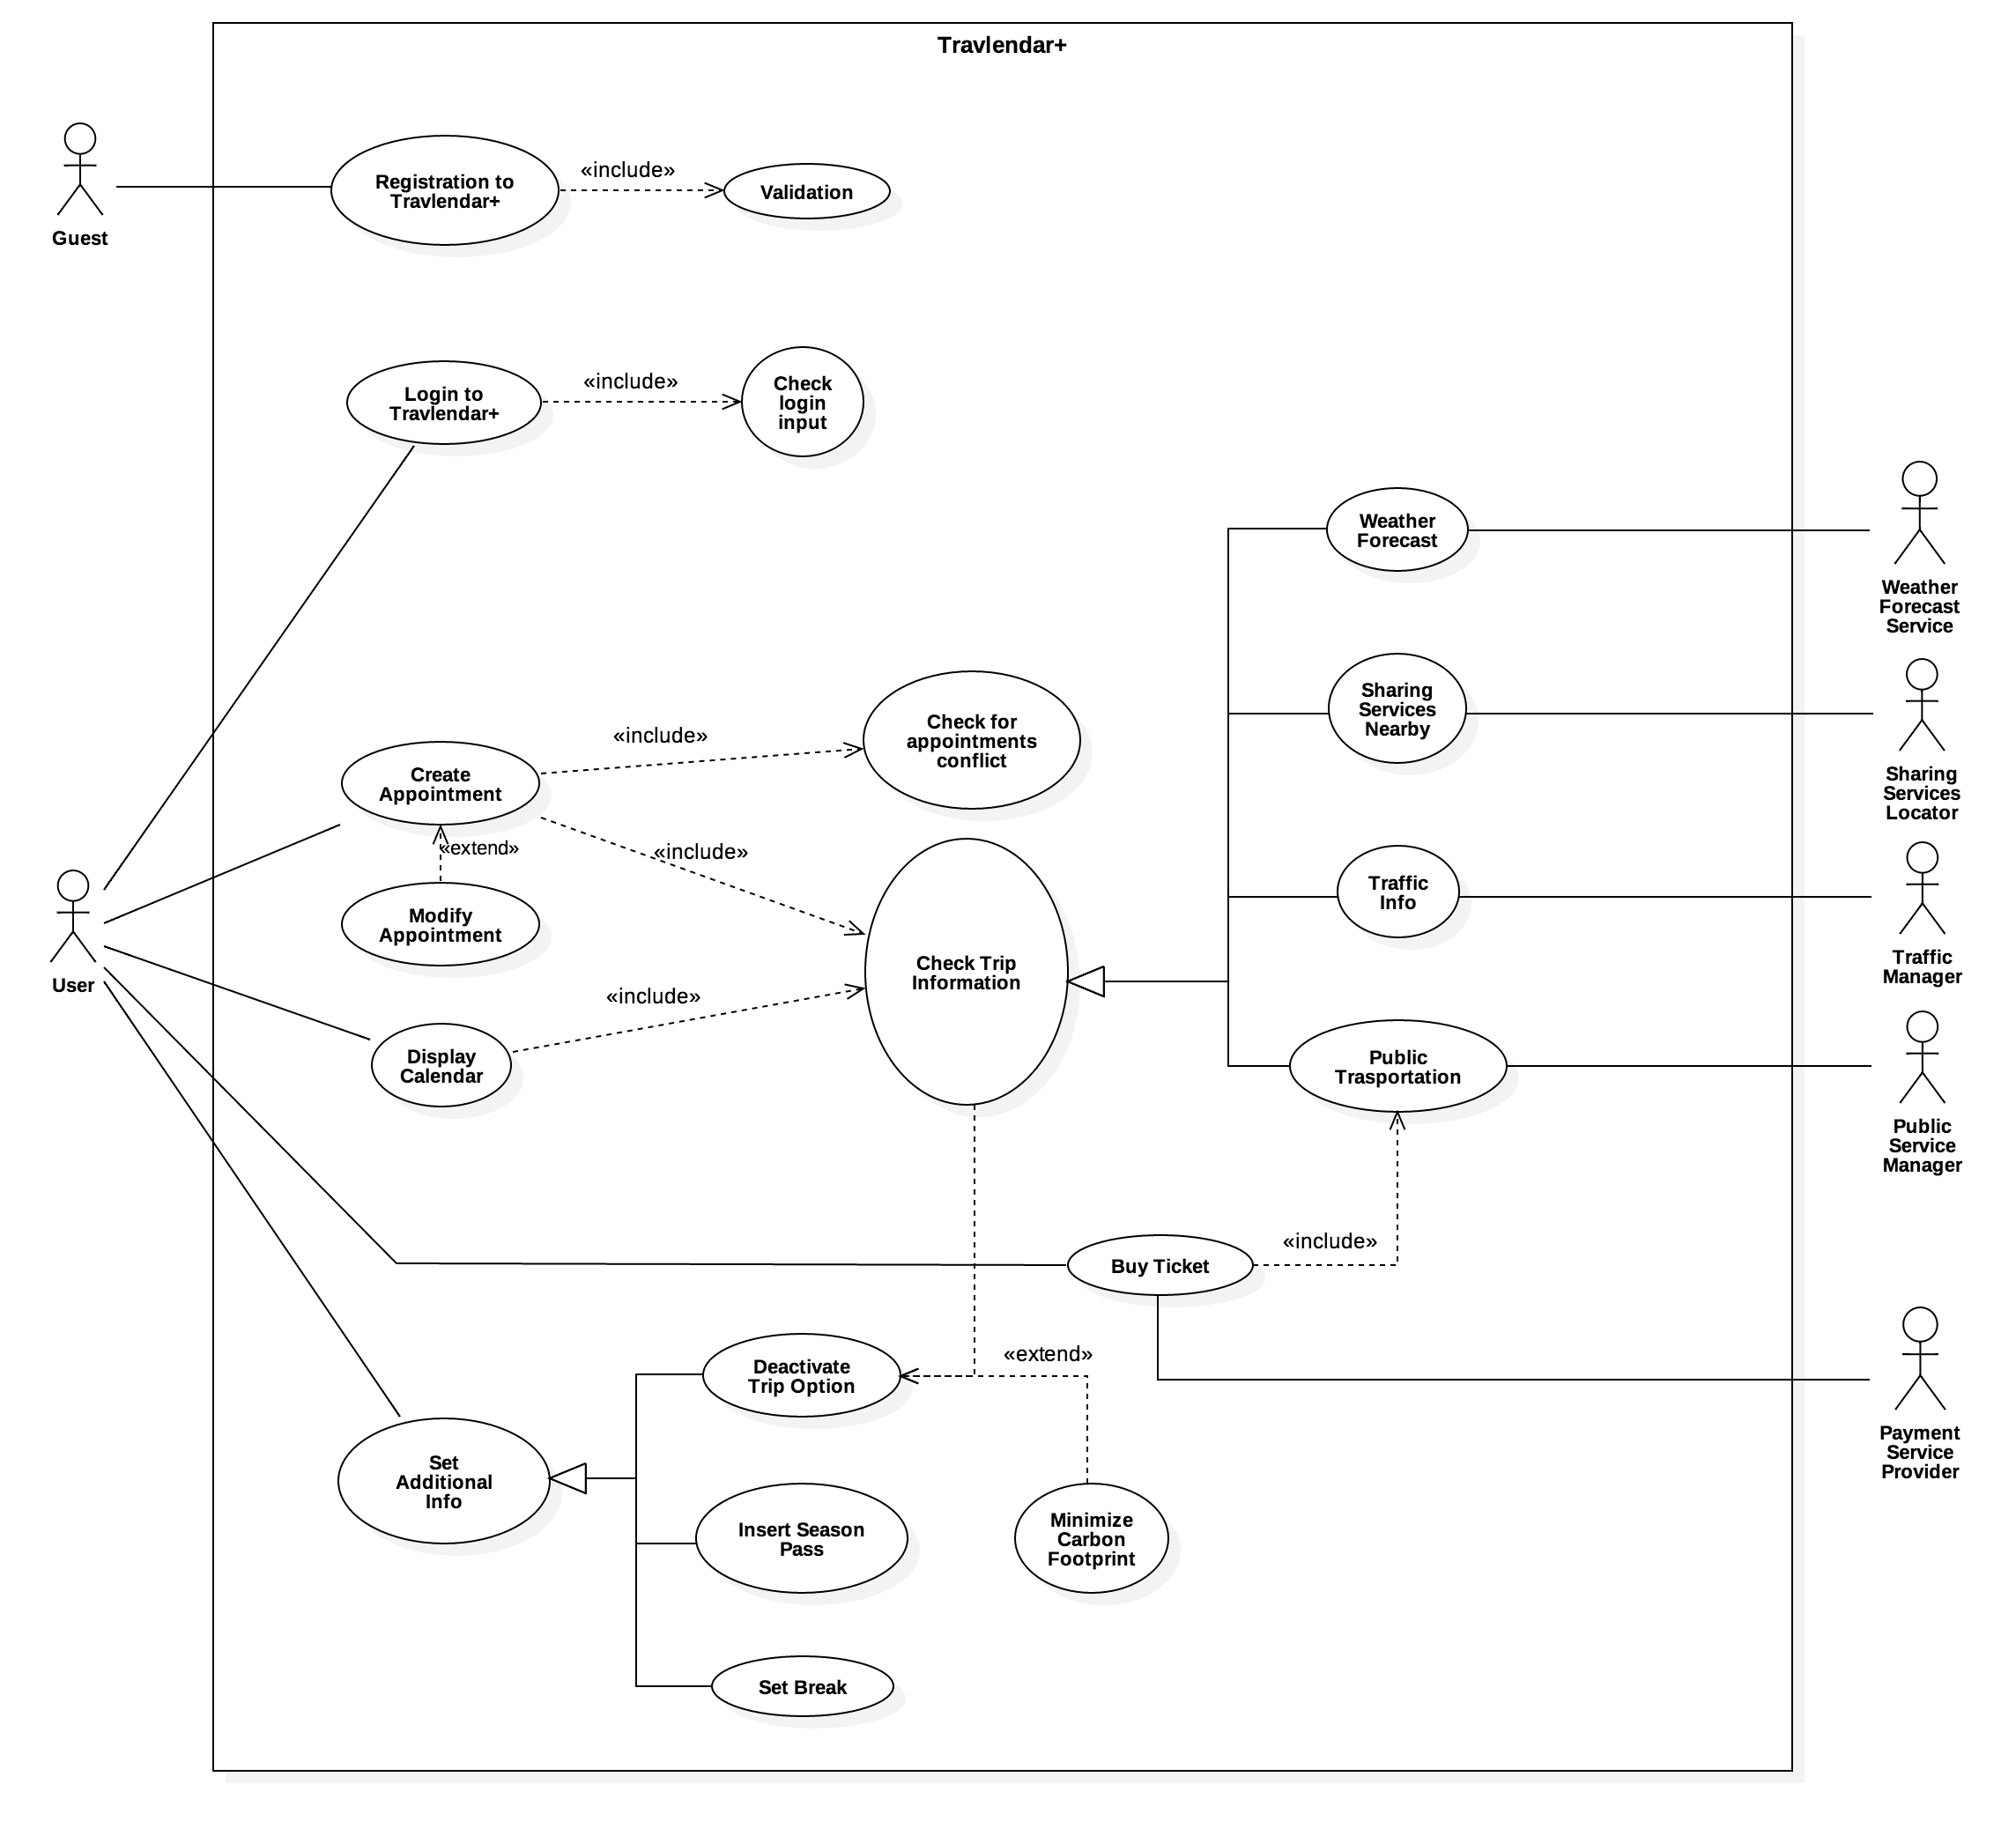
\includegraphics[width=\textwidth]{uml/useCase}

%%% REGISTER %%%	
	\paragraph{Guest registers to \textit{Travlendar+}} \label{register_useCase}
	
		\begin{tabular}{| l | p{0.8\textwidth} | }
			\hline
			\hline
			Actor	&		Guest. \\
			\hline
			Input Condition		&		NULL. \\
			\hline
			Event Flow		&		\begin{enumerate}
												\item Guest clicks on "\textit{Sign Up} button".
												\item Guest fills in at least all mandatory fields.
												\item Guest reads and accepts privacy policies and agreements from the company.
												\item Guest clicks on \textit{Confirm} button.
												\item System sends Guest a confirmation link to the provided e-mail.
												\item Guest clicks on the confirmation link.
												\item	 System saves the data in the DB.
											\end{enumerate} \\
			\hline
			Output Condition		&		Guest succesfully ends registration process and become a User. From now on he/she can log in to the application using his/her credential and start using \textit{Tralvendar+}. \\
			\hline		
			Exception		&		\begin{itemize}
											\item[-] Guest is already a User.
											\item[-] One or more mandatory fields are not valid.
											\item[-] Choosen username is already in use.
											\item[-] Email choosen is already associated to another user.
										\end{itemize}
										All exception are handle alerting the visitor of the problem and application goes back to point 2 of Event Flow \\
			\hline
			\hline
		\end{tabular}

%%% LOGIN %%%	
	\paragraph{Guest logins into \textit{Travlendar+}} \label{login_useCase}
	
		\begin{tabular}{| l | p{0.8\textwidth} | }
			\hline
			\hline
			Actor	&		Guest, User. \\
			\hline
			Input Condition		&		Guest is registered to  \textit{Travlendar+}. \\
			\hline
			Event Flow		&		\begin{enumerate}
												\item Guest fill login mandatory fields.
												\item Guest clicks on \textit{Log In} button.
												\item System verifies login credentials.
											\end{enumerate} \\
			\hline
			Output Condition		&		Guest is promoted to User and is shown is \textit{Calendar} home page. \\
			\hline		
			Exception		&		Login credentials are incorrect and Guest is shows again \textit{Login} page\\
			\hline
			\hline
		\end{tabular}

%%% CREATE A NEW EVENT %%%	
	\paragraph{Create a New Event} \label{createEvent_useCase}
	
		\begin{tabular}{| l | p{0.8\textwidth} | }
			\hline
			\hline
			Actor	&		User. \\
			\hline
			Input Condition		&		User is already logged in into \textit{Travlendar+}. \\
			\hline
			Event Flow		&		\begin{enumerate}
												\item User click on "\textit{Create Event}".
												\item User name, sets day, time and position of the Event.
												\item System checks if the new event overlaps with already existing events or break period.
												\item	 System calculates, ranks and shows multiple solutions depending on user travelling preferences.
												\item User selects one solution as preferend one.
											\end{enumerate} \\
			\hline
			Output Condition		&		\textit{Tralvendar+} shows calendar main page with the new event. \\
			\hline		
			Exception		&		\begin{itemize}
											\item[-] Created event overlaps with already existing events.
											\item[-] There are no feasible solution.
											\item[-] Inserted location isn't in the \textit{Operative Zone}.
										\end{itemize} \\
			\hline
			\hline
		\end{tabular}


%%% MODIFY EVENT %%%

	\paragraph{Modify Event}
	
		\begin{tabular}{| l | p{0.8\textwidth} | }
			\hline
			\hline
			Actor	&		User. \\
			\hline
			Input Condition		&		\begin{itemize}
													\item[-] User is already logged in into \textit{Travlendar+}.
													\item[-] Event already exists.
												\end{itemize} \\
			\hline
			Event Flow		&		\begin{enumerate}
												\item User click on "\textit{Event}".
												\item User starts modifying process.
												\item System checks if the new event overlap with already existing events or break period.
												\item	 System calculates, ranks and shows multiple solution depending on user travelling preferences.
												\item User selects one solution as preferend one.
											\end{enumerate} \\
			\hline
			Output Condition		&		\textit{Tralvendar+} shows calendar main page, with the updated event. \\
			\hline		
			Exception		&		\begin{itemize}
											\item[-] Modified event overlaps with already existing events.
											\item[-] There are no more feasible solutions.
											\item[-] Modified location is no more in the \textit{Operative Zone}.
										\end{itemize} \\
			\hline
			\hline
		\end{tabular}
		
		
%%% INSERT PAYMENT METHOD%%%

	\paragraph{Insert Payment Method}
	
		\begin{tabular}{| l | p{0.8\textwidth} | }
			\hline
			\hline
			Actor	&		User. \\
			\hline
			Input Condition		&		\begin{itemize}
													\item[-] User is already logged in into \textit{Travlendar+}.
													\item[-] Credit Card isn't already inserted on the system.
												\end{itemize} \\
			\hline
			Event Flow		&		\begin{enumerate}
												\item User click on "\textit{Preferences/Payment Methods}".
												\item User sets all the credit cards info.
												\item System checks and validate provided informations.
											\end{enumerate} \\
			\hline
			Output Condition		&		\textit{Tralvendar+} returns to \textit{Payment Methods} page showing added card as a valid payment method. \\
			\hline		
			Exception		&		Credit card given informations are invalid. \\
			\hline
			\hline
		\end{tabular}

%%% BUY TICKET %%%

	\paragraph{Buy Public Transportation Ticket} \label{buyTicket_useCase}
	
		\begin{tabular}{| l | p{0.8\textwidth} | }
			\hline
			\hline
			Actor	&		User. \\
			\hline
			Input Condition		&		\begin{itemize}
													\item[-] User is already in \textit{Solutions} page.
													\item[-] A \textit{payment method} is already available.
												\end{itemize} \\
			\hline
			Event Flow		&		\begin{enumerate}
												\item User clicks on desired solution.
												\item User clicks on "\textit{Buy Ticket} buttos".
												\item System shows available public trasportation tickets.
												\item User selects a ticket.
												\item	 System starts purchase transaction.
											\end{enumerate} \\
			\hline
			Output Condition		&		Based on public transportation service, User receives a valid ticket. \\
			\hline		
			Exception		&		\textit{External Transaction Service} doesn't worked as expected. \\
			\hline
			\hline
		\end{tabular}

%%%  RESERVE SHARING SERVICE %%%

	\paragraph{Reserve a \textit{Sharing Service} resource} \label{sharing_useCase}
	
		\begin{tabular}{| l | p{0.8\textwidth} | }
			\hline
			\hline
			Actor	&		User. \\
			\hline
			Input Condition		&		\begin{itemize}
													\item[-] User is already in \textit{Solutions} page.
													\item[-] A \textit{Sharing mean} is already available.
													\item[-] A \textit{payment method} is already available.
													\item[-] User is in the \textit{influence zone}
												\end{itemize} \\
			\hline
			Event Flow		&		\begin{enumerate}
												\item System connects to available \textit{Sharing Service} resources.
												\item System ranks per distance all the freasible recources and shows them on a map centered on User position.
												\item User chooses one on the possible solutions.												
												\item User clicks on "\textit{Reserve it} button".
												\item	 System reconnects to selected \textit{Sharing Service}, and starts the reserving procedure.
											\end{enumerate} \\
			\hline
			Output Condition		&		User redirected to the \textit{Reservation Service} app. \\
			\hline		
			Exception		&		\textit{Reservation Service} doesn't worked as expected. \\
			\hline
			\hline
		\end{tabular}
		
		
%%%  SET TRIP PREFERENCES%%%

	\paragraph{Set Trip Preferences}
	
		\begin{tabular}{| l | p{0.8\textwidth} | }
			\hline
			\hline
			Actor	&		User. \\
			\hline
			Input Condition		&		User is already logged in into \textit{Travlendar+}. \\
			\hline
			Event Flow		&		\begin{enumerate}
												\item User click on "\textit{Preferences/Trip}".
												\item System shows all the possible preferences.
												\item User pins prefered options.
											\end{enumerate} \\
			\hline
			Output Condition		&		\begin{itemize}
													\item[-] User returns to Caledar page.
													\item[-] System recalculate all future trip solution according to User preferences.
													\item[-] User is informed of particular problem
												\end{itemize} \\
			\hline
			Exception		&		User unpins all the possible preferences. \\
			
			\hline
			\hline
		\end{tabular}
		
		
%%%  SET BREAK %%%

	\paragraph{Set Break Period}
	
		\begin{tabular}{| l | p{0.8\textwidth} | }
			\hline
			\hline
			Actor	&		User. \\
			\hline
			Input Condition		&		User is already logged in into \textit{Travlendar+}. \\
			\hline
			Event Flow		&		\begin{enumerate}
												\item User click on "\textit{Preferences/Breaks}".
												\item User select an interval and a minimum lenght for his break.
											\end{enumerate} \\
			\hline
			Output Condition		&		System adds those hours as a special meeting every day in the calendar. \\
			\hline
			\hline
		\end{tabular}
